
\documentclass[xcolor={usenames,dvipsnames},12pt,presentation,aspectratio=169]{beamer}

\usepackage[utf8]{inputenc}
\usepackage[brazilian]{babel}
\usepackage{verbatim}
\usepackage{graphicx}
\usepackage{xspace}
\usepackage{amsthm}
\usepackage{url}
\usepackage{array}
\usepackage{hyperref}
\usepackage{times,mathptmx}
\usepackage{pdfpages}
\usepackage{mdframed}
\usepackage{tikz}
\usepackage{alltt}
%\usepackage[usenames,dvipsnames]{xcolor}
%\usepackage[usenames,dvipsnames]{color}
%\usepackage{color}

\usetikzlibrary{arrows,shapes}

\usetheme{Madrid}
%\usetheme{Boadilla}
%\usetheme{Darmstadt}
%\usetheme{Frankfurt}
%\usetheme{CambridgeUS}
%\usetheme{AnnArbor}
%\usecolortheme{beaver}
%\usecolortheme{seahorse}
%\usecolortheme{seagull}
\usecolortheme[named=BrickRed]{structure}

\setbeamercovered{transparent}

\setbeamertemplate{footline}[frame number]
%\setbeamertemplate{navigation symbols}{}
%\setbeamersize{text margin left=1em,text margin right=1em}

\newcommand{\titulo}{Alocação Dinâmica de Memória}
\newcommand{\disciplina}{ELC1067 - Laboratório de Programação II}
\newcommand{\nome}{João Vicente Ferreira Lima (UFSM)}

\lecture[1]{\aula}{aula01}
\def\lecturename{\aula}

\newcommand{\Red}[1]{{\color{red}#1}}
\newcommand{\red}[1]{{\color{red}#1}}
\newcommand{\Blue}[1]{{\color{blue}#1}}
\newcommand{\blue}[1]{{\color{blue}#1}}

\newcommand{\PBS}[1]{\let\temp=\\#1\let\\=\temp}
\newcommand{\RRCOL}{\PBS\raggedright\hspace{0pt}}

\newcommand{\p}[1]{\texttt{#1}}
\newenvironment{code}{%
  \begin{alltt}%
  }{%
  \end{alltt}%
}

\makeatletter
%\setbeamertemplate{headline}{}
% {%
%   \leavevmode%
%   \@tempdimb=2.4375ex%
%   \ifnum\beamer@subsectionmax<\beamer@sectionmax%
%     \multiply\@tempdimb by 4%
%   \else%
%     \multiply\@tempdimb by\beamer@subsectionmax%
%   \fi%
%   \ifdim\@tempdimb>0pt%
%     \advance\@tempdimb by 1.125ex%
%     \begin{beamercolorbox}[wd=.5\paperwidth,ht=\@tempdimb]{section in head/foot}%
%       \vbox to\@tempdimb{\vfil\insertsectionnavigation{.5\paperwidth}\vfil}%
%     \end{beamercolorbox}%
%     \begin{beamercolorbox}[wd=.45\paperwidth,ht=\@tempdimb]{subsection in head/foot}%
%       \vbox
%       to\@tempdimb{\vfil\insertsubsectionnavigation{.45\paperwidth}\vfil}%
%     \end{beamercolorbox}%
%     \begin{beamercolorbox}[wd=.05\paperwidth,ht=\@tempdimb]{subsection in head/foot}%
%       \vbox
%       to\@tempdimb{\vfil\hfil\insertframenumber\vfil\vfil}%
%     \end{beamercolorbox}%
%   \fi%
% }

\def\dohead{\beamer@headcounter=4\relax\beamer@headcounter=1\loop\ifnum\beamer@headcounter<\beamer@totalheads%
  \advance\beamer@headcounter by1\relax%
  \csname @@head\the\beamer@headcounter\endcsname\repeat}

\makeatother

\title[\titulo]{\titulo}

\subtitle{\disciplina}

\author[João V. F. Lima]{\nome}

\institute[UFSM]{Departamento de Linguagens e Sistemas de Computação \\ Universidade Federal de Santa Maria \\ \url{jvlima@inf.ufsm.br} \\ \url{http://www.inf.ufsm.br/~jvlima}}
\date{2023/1}

\graphicspath{{.}{figs/}}

\logo{ 
\includegraphics[height=1.5cm,width=1.5cm,keepaspectratio]{logo_inf}    
        
\includegraphics[height=1.5cm,width=1.5cm,keepaspectratio]{logo_ufsm} }


\newtheorem{mydef}{Definição}[section]
%\newtheorem{myteo}{Teorema}[section]
%------------------------------------------------------------------------------
%\newcommand{\xkaapi}{XKaapi\xspace}
%------------------------------------------------------------------------------
% Typesetting Listings
\usepackage{listings}
\lstset{
  language=C++,
  %basicstyle=\scriptsize\ttfamily,
 % basicstyle=\normalsize\ttfamily,
  basicstyle=\small\ttfamily,
  %basicstyle=\footnotesize\ttfamily,
  aboveskip=0pt,
  belowskip=0pt,
  mathescape=false,
  columns=flexible,
%  numbers=none,
  numbers=left,
%  showtabs=true,
%  showspaces=true,
  breaklines=true
}
%------------------------------------------------------------------------------
\lstset{commentstyle=\color{blue}}
%\lstset{stringstyle=\ttfamily}
%\lstset{ classoffset=1, 
%            morekeywords={kaapi,omp,task,data,alloca, declare, reduction, identity, parallel,sync,taskwait,cilk,spawn,tbb,css,cilk\_spawn,cilk\_sync,cilk\_for,offload},
%            keywordstyle=\color{Red}\bfseries
%           }
%\lstset{ classoffset=2, 
%            morekeywords={value,read,write,readwrite,reduction,untied,firstprivate,TaskBodyCPU,TaskBodyGPU,ka,Signature,RW,CW,range2d\_r,range2d\_rw,range2d,Spawn,Fork,Shared\_w,Shared\_r,Shared,a1,target,device,copyin,copyout,input,implements,copy\_deps,RPWP,range2d\_rpwp,rangeindex,Memory,Register,SetStaticSched,Sync,Unregister,Community,System,join\_community,SpawnMain,leave,initialize,terminate,logfile,array,SetArch,ArchHost,ArchCUDA,W,R,gpuStream,pointer\_w,pointer\_r,pointer\_cw,pointer},
%            keywordstyle=\color{Blue}\bfseries
%           }
%\lstset{ classoffset=3, 
%            morekeywords={storage,ld},
%            keywordstyle=\bfseries
%           }
%\lstset{ classoffset=4, 
%            morekeywords={in,out,inout,cout,concurrent},
%            keywordstyle=\color{Red}\bfseries
%           }
%           
\lstset{classoffset=0, showstringspaces=false}
%------------------------------------------------------------------------------
\mdfsetup{
  backgroundcolor=gray!10,
%  roundcorner=10pt,
}
%------------------------------------------------------------------------------
\newcommand{\restorefootline}{\setbeamertemplate{navigation symbols}{}}
%\newcommand{\setfootline}[1]{\setbeamertemplate{navigation symbols}{\textcolor{black}{\textbf{#1}}}}
\newcommand{\includeslides}[4]{%
  %\setfootline{#1}%
  {
    \setbeamercolor{background canvas}{bg=}
    \includepdf[pages={#2},%
    pagecommand={},
%    pagecommand={\begin{frame}[default]{}\end{frame}},
    #4,%
    turn=false,noautoscale=false,column=false,columnstrict=false,openright=false,frame=false]{#3}%
  }
  %\restorefootline%
}
%------------------------------------------------------------------------------
\begin{document}

\begin{frame}
%  \titlepage
  \maketitle
 % \mode<presentation>
 % {
 %   \begin{columns}
 %     \begin{column}{0.5\textwidth}
 %     \raggedleft
 % 
\includegraphics[width=2cm]{logo_ufsm}
 %     \end{column}
 %     \begin{column}{0.5\textwidth}
 % 
\includegraphics[width=2cm]{logo_inf}
 %     \end{column}
 %   \end{columns}
 % }
\end{frame}

\begin{frame}
    \frametitle{Outline}
    \tableofcontents[hideallsubsections]
%    \tableofcontents
\end{frame}

\AtBeginSection{
  \begin{frame}
    \frametitle{Outline}
    \tableofcontents[currentsection,hideothersubsections]
  \end{frame}
}

%%%%%%%%%%%%%%%%%%%%%%%%%%%%%%%%%%%%%%%%%%%%%%%%%%%%%%%%%%%%%%%%%%%%%%%%%%%%%%%
\section{Alocação de memória}
%%%%%%%%%%%%%%%%%%%%%%%%%%%%%%%%%%%%%%%%%%%%%%%%%%%%%%%%%%%%%%%%%%%%%%%%%%%%%%%
%------------------------------------------------------------------------------
\begin{frame}
  \frametitle{Layout de memória}
  \vspace{-3mm}
    \begin{columns}
     \begin{column}{0.7\textwidth}
    \begin{itemize}
        \item A alocação de memória é sempre contígua, tanto estático quanto dinâmico.
        \item \texttt{text} é o código da aplicação.
        \item A \textbf{pilha} (\emph{stack}) cresce do fim para o começo.
            \begin{itemize}
                \item Armazena variáveis locais
            \end{itemize}
        \item O \textbf{heap} cresce do começo ao fim.
            \begin{itemize}
                \item  Memória alocada dinamicamente
            \end{itemize}
    \end{itemize}
     \end{column}
      \begin{column}{0.3\textwidth}
  \begin{center}
	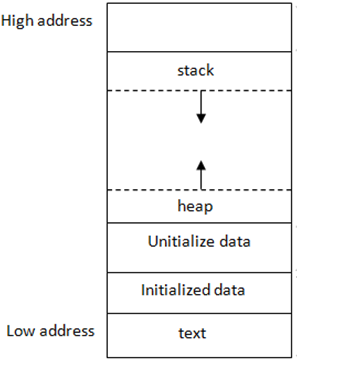
\includegraphics[width=\textwidth]{memory_layout.png}
  \end{center}
      \end{column}
    \end{columns}
\end{frame}
%------------------------------------------------------------------------------
\begin{frame}[fragile]
  \frametitle{Layout de memória}
  \begin{columns}
    \begin{column}{\textwidth}
      \begin{center}
    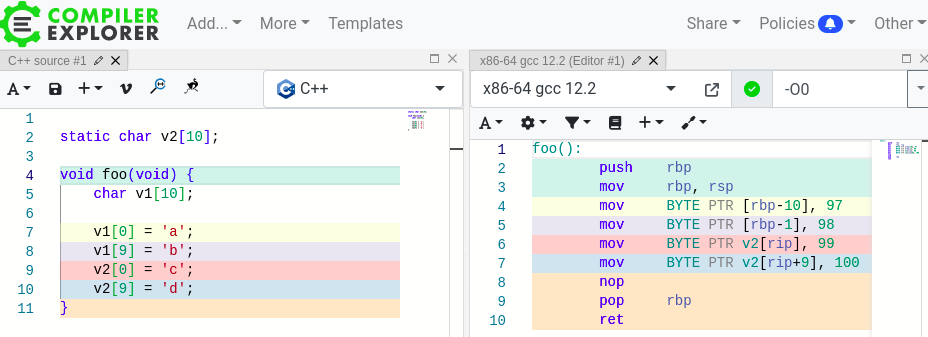
\includegraphics[width=\textwidth]{gcc.png}
      \end{center}
    \end{column}
  \end{columns}
  {\footnotesize \url{https://godbolt.org/z/envYnj8E9}}
\end{frame}
%------------------------------------------------------------------------------
\begin{frame}[fragile]
  \frametitle{Alocação de memória}
  \vspace{-2mm}
    \begin{columns}
      \begin{column}{0.55\textwidth}
\begin{block}{C}
\begin{lstlisting}
int *p = NULL;
p = (int*) malloc( sizeof(int)*10 );

*p = 1;
p[1] = 2;
*(p+2) = 3;

free( (void*)p );
\end{lstlisting}
\end{block}
     \end{column}
      \begin{column}{0.35\textwidth}
%      \begin{center}
  \begin{block}{C++}
\begin{lstlisting}
int *p = nullptr;
p = new int[10]

*p = 1;
p[1] = 2;
*(p+2) = 3;

delete[] p;
\end{lstlisting}
\end{block}
      \end{column}
    \end{columns}
  \onslide<2->
  \begin{center}
  \alert{\large \textbf{C++ não tem realloc}}
  \end{center}
\end{frame}
%%%%%%%%%%%%%%%%%%%%%%%%%%%%%%%%%%%%%%%%%%%%%%%%%%%%%%%%%%%%%%%%%%%%%%%%%%%%%%%
\section{Ponteiros}
%%%%%%%%%%%%%%%%%%%%%%%%%%%%%%%%%%%%%%%%%%%%%%%%%%%%%%%%%%%%%%%%%%%%%%%%%%%%%%%
%------------------------------------------------------------------------------
\begin{frame}[fragile]
  \frametitle{Ponteiros}
  \begin{columns}
    \begin{column}{\textwidth}
      \begin{center}
    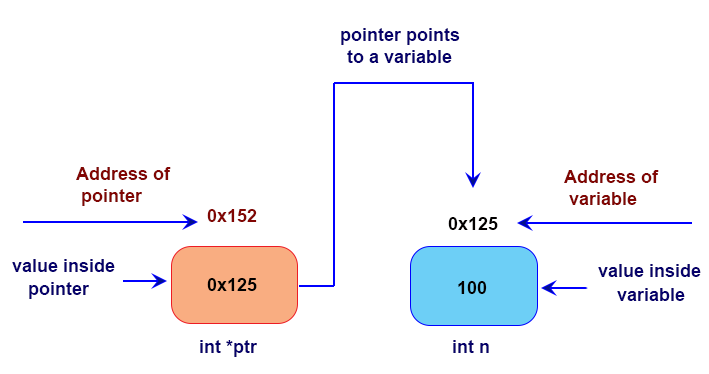
\includegraphics[width=0.8\textwidth]{c_pointer.png}
      \end{center}
    \end{column}
  \end{columns}
  {\footnotesize \url{https://www.w3resource.com/c-programming/c-pointer.php}}
\end{frame}
%------------------------------------------------------------------------------
\begin{frame}[fragile]
  \frametitle{Ponteiros}
  \begin{columns}
    \begin{column}{\textwidth}
      \begin{center}
    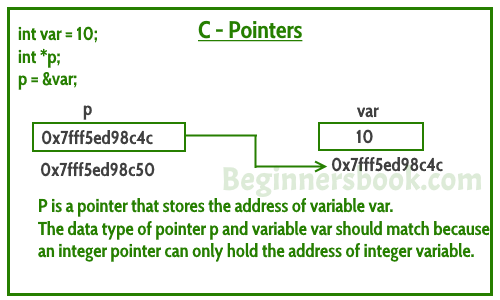
\includegraphics[width=0.7\textwidth]{pointer_memory_representation}
      \end{center}
    \end{column}
  \end{columns}
  {\footnotesize \url{https://beginnersbook.com/2014/01/c-pointers/}}
\end{frame}
%------------------------------------------------------------------------------
\begin{frame}[fragile]
  \frametitle{Matriz de caracteres}
  \begin{columns}
    \begin{column}{\textwidth}
      \begin{center}
    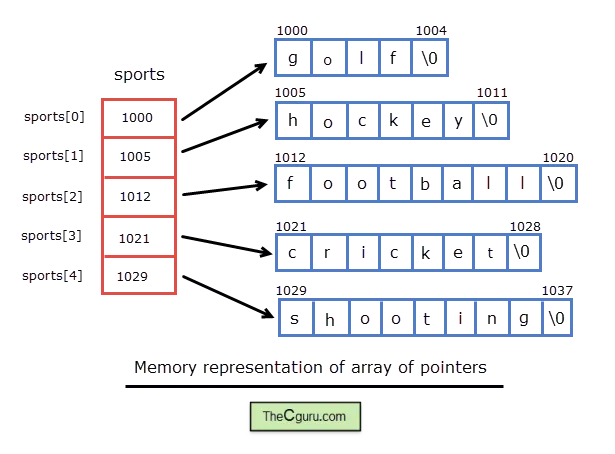
\includegraphics[width=0.7\textwidth]{C2Darray}
      \end{center}
    \end{column}
  \end{columns}
\end{frame}
%------------------------------------------------------------------------------
%------------------------------------------------------------------------------
%\begin{frame}
%  \frametitle{Entrada e saída}
%  \begin{itemize}
%  \item 
%  \end{itemize}
%\end{frame}
%------------------------------------------------------------------------------
\begin{frame}[fragile]
  \frametitle{Alocação de memória}
  \begin{block}{New e delete}
\begin{lstlisting}
int* ptr1 = nullptr;       // nullptr eh NULL em C++
int* ptr2 {nullptr};       // inicializador padrao

auto num = new int;       // aloca inteiro
*num = 33;
delete num;               // libera memoria

auto vetor = new int[10]; // vetor de 10 numeros
delete[] vetor;           // libera um vetor 

int* vetor {new int[10]}; // outra forma
delete[] vetor;
\end{lstlisting}
  \end{block}
\end{frame}
%------------------------------------------------------------------------------
%%%%%%%%%%%%%%%%%%%%%%%%%%%%%%%%%%%%%%%%%%%%%%%%%%%%%%%%%%%%%%%%%%%%%%%%%%%%%%%
\section{Matrizes}
%%%%%%%%%%%%%%%%%%%%%%%%%%%%%%%%%%%%%%%%%%%%%%%%%%%%%%%%%%%%%%%%%%%%%%%%%%%%%%%

\begin{frame}[fragile]
  \frametitle{Alocação de memória}
  \vspace{-4mm}
  \begin{block}{}
\begin{lstlisting}
int** matriz {nullptr};
int N = 10;
matriz = new int*[N];        // vetor com ponteiros
for(auto i = 0; i < N; i++)
    matriz[i] = new int[N];  // linha da matriz

// inicia valores
for(auto i = 0; i < N; i++)
    for(auto j = 0; j < N; j++)
        matriz[i][j] = 0;

// destroi matriz: cada linha e depois matriz
for(auto i = 0; i < N; i++)
    delete[] matriz[i];
delete[] matriz;
\end{lstlisting}
\end{block}
\end{frame}
%------------------------------------------------------------------------------
%%%%%%%%%%%%%%%%%%%%%%%%%%%%%%%%%%%%%%%%%%%%%%%%%%%%%%%%%%%%%%%%%%%%%%%%%%%%%%%
\section{Valgrind}
%%%%%%%%%%%%%%%%%%%%%%%%%%%%%%%%%%%%%%%%%%%%%%%%%%%%%%%%%%%%%%%%%%%%%%%%%%%%%%%
%------------------------------------------------------------------------------
\begin{frame}[fragile]
  \frametitle{Valgrind}
  \textbf{Valgrind} é uma ferramenta de depuração e instrumentação
  de programas para análise de memória.
  \begin{block}{Exemplo}
\begin{lstlisting}
int main(void)
{
    auto vetor = new int[100];
    for(auto i= 0; i < 100; i++)
        vetor[i] = 1;
    delete[] vetor;
    return 0;
}
\end{lstlisting}
\end{block}
%
  \begin{alertblock}{Execução}
\begin{lstlisting}
$ valgrind --leak-check=full ./exemplo
\end{lstlisting}
\end{alertblock}
\end{frame}
%------------------------------------------------------------------------------
\begin{frame}[fragile]
  \frametitle{Valgrind}
  \begin{block}{Saída (correto)}
\begin{lstlisting}
HEAP SUMMARY:
    in use at exit: 72,704 bytes in 1 blocks
  total heap usage: 2 allocs, 1 frees, 73,104 bytes allocated

LEAK SUMMARY:
   definitely lost: 0 bytes in 0 blocks
   indirectly lost: 0 bytes in 0 blocks
     possibly lost: 0 bytes in 0 blocks
   still reachable: 72,704 bytes in 1 blocks
        suppressed: 0 bytes in 0 blocks

ERROR SUMMARY: 0 errors from 0 contexts (suppressed: 0 from 0)
\end{lstlisting}
\end{block}
\end{frame}
%------------------------------------------------------------------------------
\begin{frame}[fragile]
  \frametitle{Valgrind}
  \begin{block}{Exemplo com erro 1}
\begin{lstlisting}
int main(void)
{
    auto vetor = new int[100];

    for(auto i= 0; i < 100; i++)
        vetor[i] = 1;

    delete vetor;

    return 0;
}
\end{lstlisting}
\end{block}
\end{frame}
%------------------------------------------------------------------------------
\begin{frame}[fragile]
  \frametitle{Valgrind}
  \vspace{-5mm}
  \begin{block}{Saída (erro 1)}
\begin{lstlisting}
Mismatched free() / delete / delete []
   at 0x4C2C2BC: operator delete(void*) (in ...)
   by 0x4007B4: main (in /home/jvlima/alloc2)
 Address 0x5a37c80 is 0 bytes inside a block of size 400 alloc'd
   at 0x4C2B800: operator new[](unsigned long) (in ...)
   by 0x400777: main (in /home/jvlima/alloc2)

HEAP SUMMARY:
    in use at exit: 72,704 bytes in 1 blocks
  total heap usage: 2 allocs, 1 frees, 73,104 bytes allocated

LEAK SUMMARY:
   definitely lost: 0 bytes in 0 blocks
   indirectly lost: 0 bytes in 0 blocks
     possibly lost: 0 bytes in 0 blocks
   still reachable: 72,704 bytes in 1 blocks
        suppressed: 0 bytes in 0 blocks
\end{lstlisting}
\end{block}
\end{frame}
%------------------------------------------------------------------------------
\begin{frame}[fragile]
  \frametitle{Valgrind}
  \begin{block}{Exemplo com erro 2}
\begin{lstlisting}
int main(void)
{
    auto vetor = new int[100];

    for(auto i= 0; i < 100; i++)
        vetor[i] = 1;

    return 0;
}
\end{lstlisting}
\end{block}
\end{frame}
%------------------------------------------------------------------------------
\begin{frame}[fragile]
  \frametitle{Valgrind}
  \begin{block}{Saída (erro 2)}
\begin{lstlisting}
HEAP SUMMARY:
    in use at exit: 73,104 bytes in 2 blocks
  total heap usage: 2 allocs, 0 frees, 73,104 bytes allocated

LEAK SUMMARY:
   definitely lost: 400 bytes in 1 blocks
   indirectly lost: 0 bytes in 0 blocks
     possibly lost: 0 bytes in 0 blocks
   still reachable: 72,704 bytes in 1 blocks
        suppressed: 0 bytes in 0 blocks
\end{lstlisting}
\end{block}
\end{frame}
%------------------------------------------------------------------------------
\begin{frame}[fragile]
  \frametitle{Valgrind}
  \begin{block}{Exemplo com erro 3}
\begin{lstlisting}
int main(void)
{
    auto vetor = new int[100];

    for(auto i= 0; i < 101; i++)
        vetor[i] = 1;
    
    return 0;
}
\end{lstlisting}
\end{block}
  \onslide<2->
  \alert{\large \textbf{Causa segmentation fault?}}
\end{frame}
%------------------------------------------------------------------------------
\begin{frame}[fragile]
  \frametitle{Valgrind}
  \begin{block}{Saída (erro 3)}
\begin{lstlisting}
==1651898== Invalid write of size 4
==1651898==    at 0x109184: main (erro.cpp:5)
==1651898==  Address 0x4dbfe10 is 0 bytes after a block of size 400 alloc'd
==1651898==    at 0x483C583: operator new[](unsigned long) (in /usr/lib/x86_64-linux-gnu/valgrind/vgpreload_memcheck-amd64-linux.so)
==1651898==    by 0x10915E: main (erro.cpp:3)
\end{lstlisting}
\end{block}
  \alert{\large Causa segmentation fault? \textbf{Não!!!}}
\end{frame}
%------------------------------------------------------------------------------
\begin{frame}[plain]{}
  \begin{center}
    \vspace{2cm}
    \Large{https://joao-ufsm.github.io/l22023a/}
    
    \vspace{1cm}
    
\includegraphics[width=2cm]{logo_ufsm}
    \hspace{0.5cm}
    
\includegraphics[width=2cm]{logo_inf}
  \end{center}
\end{frame}
%------------------------------------------------------------------------------

\end{document}
